% Main document: single-column academic article, ready for pdfLaTeX + BibTeX.
% In Overleaf, select main.tex as the main document and pdfLaTeX as compiler.
% This is a course-project paper, not a CVPR submission.
\documentclass[11pt,letterpaper]{article}

\usepackage[T1]{fontenc}
\usepackage[utf8]{inputenc}
\usepackage[margin=1in]{geometry}
\usepackage{amsmath,amssymb}
\usepackage{newtxtext,newtxmath}
\usepackage{microtype}
\usepackage{graphicx}
\usepackage{booktabs,tabularx,array}
\usepackage{caption}
\usepackage[numbers,sort&compress]{natbib}
\usepackage{xcolor}
\definecolor{linkblue}{RGB}{30,75,110}
\usepackage[colorlinks=true,allcolors=linkblue,breaklinks=true]{hyperref}
\hypersetup{
  pdftitle={Shopping History and Candidate Competition in Next Basket Recommendation},
  pdfauthor={AIAA3111 team details pending},
  pdfsubject={Single-column course-project research paper}
}
\captionsetup{font=small,labelfont=bf}
\setlength{\emergencystretch}{2em}
\setlength{\parskip}{0.25em}
\setlength{\parindent}{1.25em}
\renewcommand{\arraystretch}{1.15}
\graphicspath{{figures/}}

% Replace this author block with the actual group, members, and student IDs.
\title{Shopping History and Candidate Competition\\
in Next Basket Recommendation}
\author{AIAA3111 Course Project\\
\small Group number, member names, and student IDs to be completed}
\date{\small Team review draft}

\newcommand{\R}{\mathcal{R}}
\newcommand{\C}{\mathcal{C}}
\newcommand{\Uplus}{\mathcal{U}_{+}}
\newcommand{\Recall}{\operatorname{Recall}}
\newcommand{\TopItems}{\operatorname{Top}}
\newcommand{\pp}{\,\text{pp}}

\begin{document}
\maketitle

\begin{abstract}
Purchase histories provide both ranking signals and the catalog of products eligible for recommendation. We separate these roles in an Instacart repeat-purchase task while keeping users and true targets fixed. A fresh cohort contains 20,000 training, 5,000 validation, and 8,000 confirmation users. Among 2,526 long-history users with nonempty repeat targets, expanding the candidate pool from recent purchases to all historical products reduces Recall@10 by 3.29 percentage points under cumulative frequency but improves it by 0.47 points under time decay. A validation-selected policy retains products from the last five orders plus up to five older frequent products, reducing total candidate volume by 44.79\%. Its confirmation Recall@10 is 58.171\%, compared with 58.164\% for the full pool, meeting a prespecified 0.5-point noninferiority margin. Subsequent posthoc analysis finds unchanged mean recall for 99.45\% of eligible users. Excluded true targets mostly occupy low original ranks, and recall losses grow for longer recommendation lists. The contribution is a controlled empirical analysis of historical information, candidate competition, and the limits of selective retention.
\end{abstract}

\noindent\textbf{Keywords:} next-basket recommendation; repeat purchases; candidate selection; temporal information; evaluation.

\section{Introduction}
\label{sec:intro}

A grocery recommender must choose a short list from a user's past purchases. Retaining more history can reveal recurring preferences, but it also allows more old products to compete for limited positions. An aggregate prediction score does not distinguish these effects. Moreover, users with longer observed histories tend to have larger historical catalogs, complicating comparisons between history-length groups.

Earlier experiments in this project established strong personal-history baselines. Time weighting helped prediction, whereas adding clustering and association-rule features did not reliably improve the full model. These findings motivated three research questions. First, how sensitive are history-group comparisons to differences in task composition? Second, what happens when scoring history and candidate eligibility change separately? Third, how much candidate reduction can a fixed short-list ranker tolerate, and where does the resulting performance claim stop applying?

We address these questions using a fixed-target evaluation. A policy may remove products from the eligible candidate pool, but it cannot remove those products from the true repeat-target set used to evaluate recommendations. A factorial experiment then changes the history used for scoring independently of the products allowed to compete. Finally, a validation-selected policy is frozen and tested on previously unused confirmation users. A subsequent, explicitly posthoc analysis examines individual changes and recommendation depth.

The contribution is empirical and methodological. We demonstrate that the effects of old candidates depend on scoring, quantify recovered and displaced true hits, and identify a candidate-reduction policy that retains average Top~10 recall within a declared tolerance. We also show why this result is narrow: most short lists remain unchanged, while excluded true targets become reachable in longer full-pool lists. We do not propose a new state-of-the-art algorithm or infer how shoppers psychologically forget products.

\subsection{Relation to prior work}
TIFU-KNN models personalized item frequency with temporal weighting and information from neighboring users~\citep{hu2020}. A next-basket recommendation reality check distinguishes repeat and exploratory recommendation and emphasizes the importance of task definition and evaluation~\citep{li2023}. These established ideas inform our task and baselines; we do not claim to introduce the repeat--explore distinction. We use LightGBM~\citep{ke2017} as a learned ranker and compare an independently written adaptation of TIFU-KNN in an earlier cohort. The present study focuses on separating ranking information from candidate competition and on explaining performance retention through exact hit accounting.

\section{Task and Evidence Design}
\label{sec:task}

\subsection{Data and prediction boundary}
The public Instacart dataset contains 206,209 users, 3,421,083 orders, and 49,688 products. Six CSV files provide order sequences, basket contents, and product metadata~\citep{instacart2017,kaggle}. The eligible labeled population comprises 131,209 users whose terminal order has released product labels; our study cohorts are sampled from this population. Earlier orders form each user's observed history. Prediction takes place after the last historical order, before any metadata from the terminal order is available.

Let $\C_{\mathrm{all}}(u)$ be the set of products purchased in user $u$'s observed history and $B_{\mathrm{next}}(u)$ the terminal basket. The fixed repeat-target set is
\begin{equation}
  \R(u)=B_{\mathrm{next}}(u)\cap\C_{\mathrm{all}}(u).
  \label{eq:target}
\end{equation}
A policy $p$ selects an eligible subset $\C_p(u)\subseteq\C_{\mathrm{all}}(u)$ and returns up to $K$ ranked products, denoted $\TopItems_{K,p}(u)$. For $\R(u)\ne\varnothing$,
\begin{equation}
  \Recall@K(u,p)=\frac{|\TopItems_{K,p}(u)\cap\R(u)|}{|\R(u)|},\qquad
  \overline{\Recall}@K(p)=\frac{1}{|\Uplus|}\sum_{u\in\Uplus}\Recall@K(u,p),
  \label{eq:recall}
\end{equation}
where $\Uplus$ contains users with nonempty full-history repeat targets. Excluded true products remain in $\R(u)$ and can therefore remain misses. Candidate pruning never changes the targets or user population.

The main confirmation sample has 8,000 users, including 528 with empty repeat targets. Thus 7,472 contribute to macro recall and NDCG. Empty-target users remain in counts, precision, and F1; their recall is undefined rather than zero. We also record hits divided by $K$, actual recommendation length, candidate coverage, and the candidate-constrained Top-$K$ oracle. This distinguishes changes in eligibility and returned list length from changes in achieved retrieval.

\subsection{Separate exploration from confirmation}
Table~\ref{tab:cohorts} summarizes the evidence stages. The four user cohorts are mutually disjoint. The final memory study excludes all 76,000 users used in earlier stages before sampling a fresh cohort of 33,000. Scores from different cohorts are not interpreted as a chronological improvement curve. The follow-up uses completed confirmation predictions and is not an additional independent test.

\begin{table}[tbp]
  \centering
  \caption{Evidence stages and user counts. The posthoc follow-up reuses the final confirmation cohort without fitting new models or choosing a new policy.}
  \label{tab:cohorts}
  \small
  \begin{tabularx}{\linewidth}{@{}lrrrX@{}}
    \toprule
    Stage & Training & Validation & Held out & Role \\
    \midrule
    Initial study & 7,000 & 1,500 & 1,500 & Pipeline and hypotheses \\
    Information study & 20,000 & 5,000 & 8,000 & Feature comparisons \\
    Baseline extension & 20,000 & 5,000 & 8,000 & TIFU and robustness \\
    Memory study & 20,000 & 5,000 & 8,000 & Main confirmation \\
    Posthoc follow-up & --- & --- & Same 8,000 & Interpretation and scope \\
    \bottomrule
  \end{tabularx}
\end{table}

Global statistics, clustering, association rules, and neighbor banks use training users' historical data only. Held-out users supply their own past purchases and do not enter other held-out users' neighbor banks. No terminal-order day, hour, or interval enters a predictor. All historical products are candidates before policy filtering, with no negative sampling. Absolute calendar dates and prices are absent, and inter-order gaps are capped at 30 days. The experiment is therefore a within-user chronological evaluation, not a global calendar backtest or spending analysis.

\section{Methods and Evaluation}
\label{sec:methods}

\subsection{Separate scoring history from eligibility}
The core $2\times2$ design crosses the history used for scoring (recent five orders or all observed orders) with eligible candidates (products in the recent five orders or all historical products). Every cell knows the complete historical catalog and uses the same terminal targets. The experiment changes the algorithmic use of history, not how much history the user actually possesses.

For a product $i$, let $x_{u,i,t}$ indicate its presence in historical order $t$, let $T_u$ be the last observed order, and let $\mathcal{W}_u$ be the selected scoring window. Frequency and time-decayed scores are
\begin{equation}
 s_{\mathrm{freq}}(u,i)=\sum_{t\in\mathcal{W}_u}x_{u,i,t},\qquad
 s_{\mathrm{decay}}(u,i)=\sum_{t\in\mathcal{W}_u}0.8^{T_u-t}x_{u,i,t}.
 \label{eq:scores}
\end{equation}
Age is measured in orders; age zero is the latest observed order. Purchases outside a recent scoring window contribute zero. The primary factorial population has at least 16 historical orders and nonempty repeat targets: the same 2,526 users in all cells. Windows of three and ten orders are sensitivity settings.

The \emph{information contrast} adds old purchases to scoring while fixing the full candidate pool. The \emph{expansion contrast} enlarges the pool while keeping all-history scores fixed. We also report the interaction, namely the difference in the information contrast between full and recent candidate pools. Recent-window scores are zero for products outside that window. When the recent pool already contains at least $K$ positive-score products, adding zero-score old products cannot affect the Top~$K$. Some interaction structure is therefore built into the design and should not be interpreted as an unexpected behavioral discovery.

\subsection{Learned ranking and candidate policies}
A LightGBM classifier~\citep{ke2017} scores user--product pairs using frequency, recency, basket history, purchase-gap, product, and department-affinity features. The fixed settings are 240 trees, learning rate 0.05, 31 leaves, minimum child size 80, feature fraction 0.9, and an L2 penalty of 1. Models use seeds 42, 73, and 123. Policies share each fitted model's scores. We average metrics within each user across seeds before paired analysis; this is not an ensemble of prediction scores.

The selective pool keeps every product from the recent five orders and adds up to $M$ older products. Older products are ordered by all-history purchase count, then recency, then product ID. Writing $\C_5(u)$ for the recent pool and $\mathcal{O}_M(u)$ for the first $M$ ranked products in $\C_{\mathrm{all}}(u)\setminus\C_5(u)$,
\begin{equation}
 \C_{\mathrm{selected}}(u;M)=\C_5(u)\cup\mathcal{O}_M(u).
 \label{eq:policy}
\end{equation}
Validation tests $M\in\{0,5,10,20,40,80\}$. We select the smallest mean pool whose paired marginal 95\% lower confidence bound for Recall@10 relative to the full pool is at least $-0.005$, with a full-pool fallback. The selection rule is fixed before confirmation. Two controls choose products from the full historical catalog by frequency or by recency, using exactly the same candidate count as the selected policy for each user. Neither control uses target labels, and ties are deterministic.

\subsection{Uncertainty and exact hit accounting}
The main study prespecifies nine contrasts and uses 6,000 paired-user bootstrap replicates, reporting both marginal and Bonferroni simultaneous 95\% intervals. Final noninferiority requires the simultaneous lower bound for selected minus full recall to be at least $-0.005$, equivalent to $-0.5$ percentage points (pp). Validation is a selection stage; independent confirmation determines the final claim. Intervals condition on fitted models and do not include retraining uncertainty.

Under fixed scores, enlarging a candidate pool can introduce correct recommendations and displace correct recommendations from the smaller pool. Let $L_{\mathrm{small}}$ and $L_{\mathrm{large}}$ be the two Top-$K$ lists for one user. Then
\begin{align}
 g_u&=|(L_{\mathrm{large}}\setminus L_{\mathrm{small}})\cap\R(u)|, &
 \ell_u&=|(L_{\mathrm{small}}\setminus L_{\mathrm{large}})\cap\R(u)|,\nonumber\\
 \Delta\Recall@K(u)&=\frac{g_u-\ell_u}{|\R(u)|}.
 \label{eq:ledger}
\end{align}
Dividing each term by the same full target before averaging preserves exact additivity for macro recall. This ledger is an algorithmic accounting identity, not a causal model of shopper psychology.

\section{Results}
\label{sec:results}

\subsection{Earlier baselines establish the context}
Table~\ref{tab:baselines} reports selected within-cohort contrasts from the earlier information study and baseline extension. Time weighting improves a frequency baseline, and temporal features retain value conditional on other model features. Clustering and association rules show no stable overall benefit beyond the full model. An early local rule signal does not clearly replicate in the later cohort. A quota-constrained reranker selects weight zero on validation, leaving the base ranking unchanged; its equal confirmation score is a structural identity, not evidence that the proposed change succeeded.

\begin{table}[tbp]
  \centering
  \caption{Earlier within-cohort evidence. Differences are in percentage points of Recall@10. The first two rows use the information cohort; the last two use the separate baseline-extension cohort.}
  \label{tab:baselines}
  \small
  \begin{tabularx}{\linewidth}{@{}XrX@{}}
    \toprule
    Comparison & Difference & Interpretation \\
    \midrule
    Time decay minus frequency & $+3.73$ & Time information helps \\
    Full minus no temporal features & $+3.89$ & Conditional temporal value \\
    TIFU minus same-time personal vector & $+0.61$ & Small neighbor contribution \\
    Full minus adapted TIFU & $+1.96$ & Strong learned baseline \\
    \bottomrule
  \end{tabularx}
\end{table}

The independent TIFU-KNN adaptation follows documented author-code time weighting and restricts recommendations to historical candidates. It is not a reproduction of the paper's full-basket benchmark~\citep{hu2020}. Its neighbor contrast uses the same selected personal time vector. Because the rule and neighbor experiments begin from different personal baselines, their differences cannot be attributed solely to information representation.

\subsection{History-group composition changes the comparison}
In the memory study, users with 3--5 historical orders have mean Recall@10 of 67.97\%, compared with 50.11\% for users with at least 16 orders. Across all users in those groups, mean historical candidate counts are 27.66 and 111.48, respectively. The raw long-minus-short recall gap is therefore $-17.86\pp$, but the two groups differ substantially in the size of the recommendation task.

We restrict comparisons to common historical-covariate cells and apply identical pooled cell weights to each history group. Strata use either candidate count alone or candidate count together with historical mean basket size. Figure~\ref{fig:history} separates the change in population from the subsequent reweighting. Count-only strata retain 5,970 of 7,472 eligible users (79.90\%); count-plus-basket-size strata retain 3,424 (45.82\%). Same-support raw gaps remain negative at $-5.68$ and $-8.06\pp$, whereas standardized gaps are $+13.15$ and $+4.21\pp$. Their conditional marginal 95\% intervals are $[+11.10,+15.13]$ and $[+0.90,+7.15]\pp$.

\begin{figure}[tbp]
  \centering
  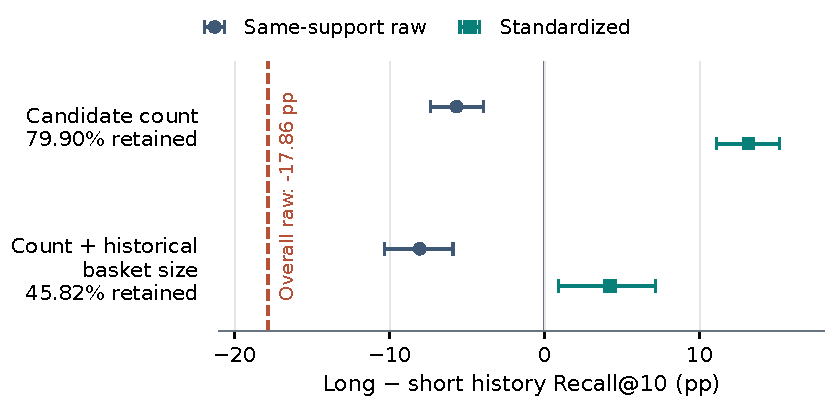
\includegraphics[width=0.95\linewidth]{history_composition.pdf}
  \caption{History-group composition diagnostic among users with nonempty repeat targets. Differences are long minus short history Recall@10. The overall raw comparison, restriction to common support, and reweighting within that support answer different questions. Bars are conditional marginal 95\% intervals, not the main nine-contrast simultaneous intervals. The cell-count thresholds of 10 and 20 yield identical support within each scheme.}
  \label{fig:history}
\end{figure}

Minimum cell counts of 10 and 20 yield identical support within each stratification scheme, so four planned settings produce only two distinct comparisons. Future target size does not define the strata, although recall still conditions inclusion on a nonempty future repeat target. Coarse bins, restricted support, and unobserved differences prevent a causal interpretation. The result demonstrates that the apparent history-length trend is sensitive to comparison composition; it does not prove that obtaining more history makes prediction easier.

\subsection{Old history helps or hurts depending on scoring}
Figure~\ref{fig:factorial} presents the factorial results for the same 2,526 long-history users. With the full candidate pool fixed, adding older purchases to scoring lowers frequency Recall@10 by $2.51\pp$ but raises decayed-frequency recall by $2.03\pp$. With all-history scores fixed, expanding candidates lowers frequency recall by $3.29\pp$ but raises decayed-frequency recall by $0.47\pp$. All four directions are supported by simultaneous intervals excluding zero (Table~\ref{tab:primary}). Thus old information and old candidates are not inherently harmful: their effects depend on how the ranking treats purchase time.

\begin{figure}[tbp]
  \centering
  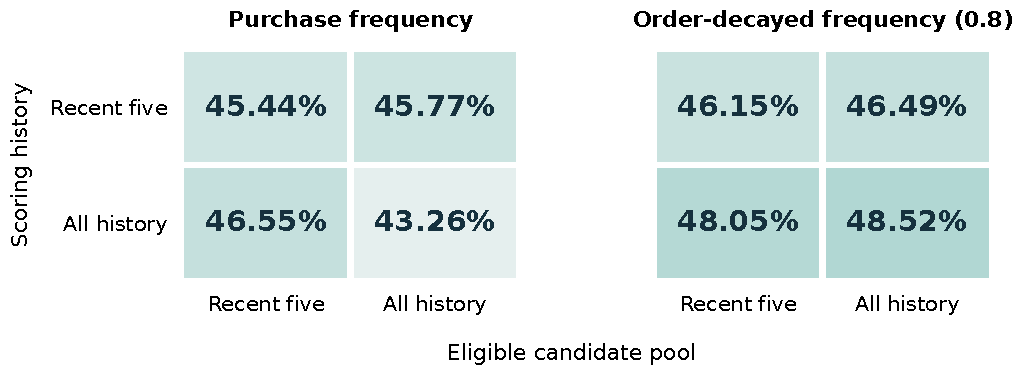
\includegraphics[width=\linewidth]{factorial_memory.pdf}
  \caption{Factorial comparison on the same 2,526 users with at least 16 historical orders and nonempty repeat targets. Rows change scoring history and columns change candidate eligibility. All cells use the complete historical catalog and fixed repeat-target denominator. Values are macro Recall@10.}
  \label{fig:factorial}
\end{figure}

\begin{table}[tbp]
  \centering
  \caption{All nine prespecified main-study contrasts. Differences and intervals are in percentage points of Recall@10. Intervals are simultaneous 95\% over the nine contrasts. The noninferiority claim concerns the selected-minus-full row and the predeclared $-0.5\pp$ margin.}
  \label{tab:primary}
  \small
  \begin{tabular}{@{}lrrr@{}}
    \toprule
    Contrast & Users & Difference & Simultaneous 95\% interval \\
    \midrule
    Frequency scoring information & 2,526 & $-2.513$ & $[-3.846,-1.163]$ \\
    Decay scoring information & 2,526 & $+2.030$ & $[+1.291,+2.734]$ \\
    Frequency candidate expansion & 2,526 & $-3.287$ & $[-4.356,-2.265]$ \\
    Decay candidate expansion & 2,526 & $+0.466$ & $[+0.139,+0.826]$ \\
    Frequency interaction & 2,526 & $-3.624$ & $[-4.639,-2.630]$ \\
    Decay interaction & 2,526 & $+0.130$ & $[-0.172,+0.435]$ \\
    \midrule
    Selected minus full & 7,472 & $+0.007$ & $[-0.066,+0.071]$ \\
    Selected minus frequency budget & 7,472 & $+0.192$ & $[+0.044,+0.342]$ \\
    Selected minus recency budget & 7,472 & $+0.061$ & $[-0.039,+0.165]$ \\
    \bottomrule
  \end{tabular}
\end{table}

The exact ledger in Table~\ref{tab:ledger} explains the net change. Frequency retrieves some old true targets, but loses more recall through displaced correct recommendations. Decay introduces fewer old products into the leading positions and achieves a positive balance. These observations reject a blanket recommendation to discard all older products. The frequency interaction is negative, while the decay interaction interval includes zero. Because recent scoring assigns zero to old products, part of the interaction is structural. We therefore emphasize fixed-score candidate expansion. The learned-model ledger is descriptive rather than an additional prespecified test.

\begin{table}[tbp]
  \centering
  \caption{Exact hit accounting for expansion from recent candidates to all historical candidates under fixed full-history scores. Each contribution is divided by the same user's full repeat-target count before averaging across the 2,526 long-history users. Learned-model contributions average three seeds. Displayed rounding can affect sums; stored per-user identities balance exactly.}
  \label{tab:ledger}
  \small
  \begin{tabularx}{\linewidth}{@{}Xrrr@{}}
    \toprule
    Scoring method & Recovered true hits & Displaced true hits & Net recall \\
    \midrule
    Frequency & $+3.66\pp$ & $-6.94\pp$ & $-3.29\pp$ \\
    Decay & $+0.61\pp$ & $-0.14\pp$ & $+0.47\pp$ \\
    Learned model & $+1.45\pp$ & $-0.58\pp$ & $+0.87\pp$ \\
    \bottomrule
  \end{tabularx}
\end{table}

\subsection{Selective retention preserves short-list performance}
Validation selects $M=5$: recent-only candidates fail the selection criterion, and adding up to five older frequent products gives the smallest tested qualifying pool. Selection, model scores, and evaluation code are frozen before confirmation. Table~\ref{tab:policies} reports the independent confirmation outcomes for this fixed policy and its controls.

\begin{table}[tbp]
  \centering
  \caption{Candidate policies on the memory-study confirmation cohort. Candidate means use all 8,000 users; Recall@10 and target coverage use the 7,472 nonempty-target users. Same-budget controls match the selected pool size separately for every user.}
  \label{tab:policies}
  \small
  \begin{tabularx}{\linewidth}{@{}Xrrr@{}}
    \toprule
    Candidate policy & Mean candidates & Recall@10 & Target coverage \\
    \midrule
    Full historical pool & 64.92 & 58.164\% & 100.00\% \\
    Recent five orders only & 32.49 & 57.674\% & 87.06\% \\
    Recent plus five old frequent & 35.85 & 58.171\% & 90.87\% \\
    Same-budget frequency & 35.85 & 57.980\% & 89.91\% \\
    Same-budget recency & 35.85 & 58.110\% & 90.48\% \\
    \bottomrule
  \end{tabularx}
\end{table}

Total eligible candidate volume decreases by 44.79\%, equivalently the reduction in the ratio of mean candidate counts for the same 8,000 users. The mean of users' individual retention ratios is 73.01\%, a different aggregation. Selected-minus-full recall is $+0.0072\pp$, with simultaneous interval $[-0.0657,+0.0713]\pp$. Its lower bound exceeds the prespecified $-0.5\pp$ margin, supporting noninferiority. The interval crosses zero, so the evidence does not establish superiority or exact equality.

\begin{figure}[tbp]
  \centering
  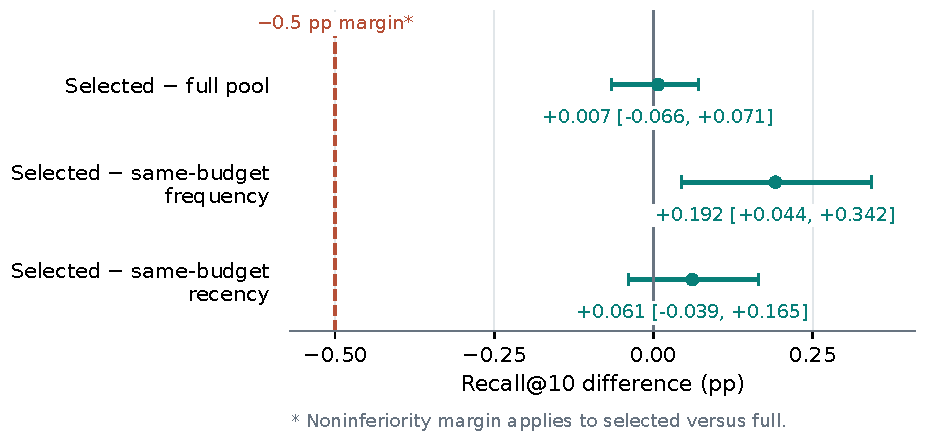
\includegraphics[width=0.95\linewidth]{policy_contrasts.pdf}
  \caption{Main-study policy contrasts on 7,472 nonempty-target users. Bars show simultaneous 95\% intervals across the nine prespecified contrasts. The $-0.5\pp$ reference applies to selected versus full noninferiority; it is not a superiority threshold for all contrasts.}
  \label{fig:policies}
\end{figure}

The selected policy exceeds same-budget frequency by $0.192\pp$, but the $0.061\pp$ difference from same-budget recency is uncertain. The result therefore supports selective retention under the tested conditions, without showing that the old-frequency rule is uniquely optimal.

\paragraph{Recall retention does not preserve all target coverage.}
Macro candidate coverage falls to 90.87\%, and the candidate-constrained oracle Recall@10 decreases from 93.34\% to 86.09\%. Excluded true targets remain in evaluation, but the current full ranker rarely retrieves them in its Top~10. Coverage loss and nearly unchanged achieved recall can consequently coexist. This does not mean the excluded products lack value.

The full model's whole-basket Recall@10 is 35.82\%, compared with 58.16\% for repeat targets. First-time product recommendation is outside this study's modeled candidate scope. In addition, full scores are computed before candidate masking, so candidate reduction does not demonstrate faster scoring, lower memory use, or end-to-end deployment savings.

\subsection{Posthoc interpretation and recommendation-depth limits}
\label{sec:posthoc}
After confirmation, we inspect the frozen predictions without fitting models or choosing new parameters. All findings in this subsection are posthoc. Among 7,472 users with nonempty repeat targets, 7,431 (99.45\%) have unchanged seed-averaged recall, 23 improve, and 18 decline. Across all 8,000 users, 96.225\% retain exactly the same ordered Top~10 under all three models. Average preservation therefore arises mainly from unchanged recommendations, rather than broad gains offsetting broad losses.

Some individuals still lose: the 18 harmed users have a conditional mean recall decline of $21.03\pp$. This outcome-selected group is not a validated prediction-time subgroup. Historical subgroup intervals do not supply stable evidence for a deployment subgroup that reliably benefits.

Of 5,274 excluded true repeat targets, only 0.26\% originally rank in the full model's Top~10, while 95.54\% rank after position 20, averaging rank-bin counts across seeds. Longer full-pool lists begin to reach these targets, making deletion losses exceed gains from promoted retained products. Figure~\ref{fig:depth} and Table~\ref{tab:depth} show all six inspected list lengths. The twelve posthoc contrasts use a separate family of simultaneous intervals; the repeated $K=10$ point is not another independent confirmation.

\begin{figure}[tbp]
  \centering
  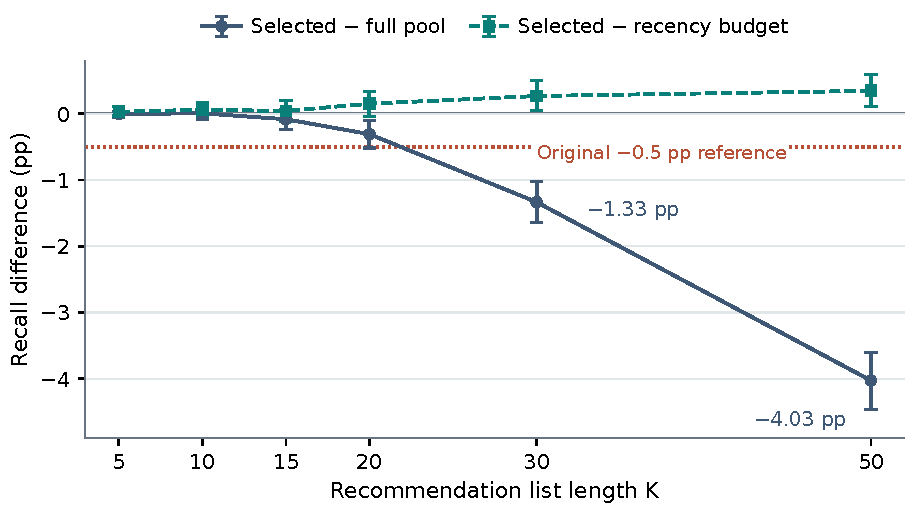
\includegraphics[width=0.95\linewidth]{list_depth.pdf}
  \caption{Posthoc recommendation-depth analysis. Policies and scores are fixed. Intervals use 6,000 paired-user bootstrap samples and simultaneous adjustment over twelve comparisons. Lines connect tested values only. The original $-0.5\pp$ margin is a reference, not a newly confirmed safe-$K$ boundary.}
  \label{fig:depth}
\end{figure}

\begin{table}[tbp]
  \centering
  \caption{All twelve posthoc depth contrasts on 7,472 nonempty-target users. Each entry reports selected-minus-comparator Recall@K in percentage points, followed by its simultaneous 95\% interval. These intervals belong to the posthoc family and differ from the original nine-contrast confirmation intervals.}
  \label{tab:depth}
  \small
  \begin{tabular}{@{}rcc@{}}
    \toprule
    $K$ & Compared with full pool & Compared with recency budget \\
    \midrule
    5  & $-0.001\;[-0.057,+0.042]$ & $+0.032\;[-0.028,+0.115]$ \\
    10 & $+0.007\;[-0.078,+0.070]$ & $+0.061\;[-0.047,+0.172]$ \\
    15 & $-0.082\;[-0.241,+0.070]$ & $+0.043\;[-0.114,+0.201]$ \\
    20 & $-0.308\;[-0.517,-0.103]$ & $+0.152\;[-0.036,+0.336]$ \\
    30 & $-1.334\;[-1.645,-1.023]$ & $+0.269\;[+0.045,+0.497]$ \\
    50 & $-4.028\;[-4.471,-3.606]$ & $+0.349\;[+0.106,+0.592]$ \\
    \bottomrule
  \end{tabular}
\end{table}

At $K=20$, the selected-minus-full interval $[-0.517,-0.103]\pp$ slightly crosses the original margin. This does not overturn the original Top~10 confirmation, and these posthoc observations do not establish a newly chosen safe cutoff. At $K=30$ and 50, losses increase to $1.334$ and $4.028\pp$.

The recency-budget control remains close partly because both policies retain all recent products. Their overall candidate Jaccard averages 92.92\%, versus 53.35\% for old-only candidates among users with a nonempty old union. For 94.61\% of all users, all three models produce identical Top~10 lists. At $K=30$ and 50, selected retention modestly exceeds recency-budget recall but still falls behind the full pool. These local advantages do not establish overall superiority, and low original ranks do not imply that a stronger model could never recover the excluded targets.

\section{Discussion and Limitations}
\label{sec:discussion}

The empirical contribution is a fixed-target comparison of historical scoring and candidate eligibility, with exact hit accounting and matched-budget controls. The findings constrain candidate reduction to the tested scoring model and recommendation depth. Average noninferiority does not protect every user or preserve target coverage. Negative rule results, the inactive quota proposal, and the competitive recency control remain part of the evidence.

Several limits constrain generalization. We study one historical platform and one terminal order per evaluated user, without an online user study, prices, or absolute calendar dates. Recommendations are restricted to previously purchased products. Standardization uses coarse bins and common support, and its intervals condition on that support and the existing fitted model. Three seeds do not replace retraining on new training samples. The individual-user and list-depth analyses are posthoc. No measured runtime, storage, sales, or satisfaction improvement is claimed. A stronger ranker could increase the value of the currently low-ranked excluded targets.

Future work should place selection before expensive scoring, measure runtime and memory, and evaluate new users or independent time periods. Adapting pools to recommendation depth or user characteristics requires a new selection-and-confirmation cycle; these improvements are not established here.

\section{Conclusion}
History supplies both ranking signals and eligible competitors. Separating these roles reveals opposite effects of old candidates under frequency and time decay. A frozen policy reduces candidate volume by 44.79\% while retaining average Recall@10 within a prespecified 0.5-point tolerance. Most short lists remain unchanged, but longer lists expose excluded targets. Candidate reduction must therefore be evaluated with fixed targets, matched-budget controls, and its intended recommendation depth.

\section*{Reproducibility and AI Assistance Disclosure}
The project preserves protocols, disjoint user splits, source hashes, validation choices, frozen predictions, evidence tables, and independent computational audits. The main study checks raw baskets and fixed-target evaluation; the follow-up reproduces rankings, hit ledgers, and intervals. The packaged research test suite passes 108 tests. These checks support implementation consistency, not external generalization. The separate source-and-evidence package README distinguishes inspecting saved evidence from reproducing full-data preparation and fitting; a clean rerun is not promised to yield byte-identical model files.

OpenAI Codex assisted research design, implementation, experiment execution, analysis, visualization, and drafting. Automated tests and computational checks were performed, but team review is still required. This document is a team review draft and does not imply that students independently authored or verified all content. Before submission, the team must review the work, revise the final expression based on its own understanding, verify references, supply actual member identities and contributions, and disclose assistance according to the course policy.


\bibliographystyle{plainnat}
\bibliography{references}

\end{document}
